\documentclass[12pt]{article}
\usepackage[utf8]{inputenc}
\usepackage[T1]{fontenc}
\usepackage[german]{babel}


\usepackage{graphicx}

%   Abbildungen müssen in einem Ordner "Abbildungen" liegen
\graphicspath{ {Abbildungen/} }
\usepackage{pdfpages}
\usepackage{csquotes}

\usepackage{etoolbox}
\AtBeginEnvironment{quote}{\small\setstretch{.25}}

\usepackage{helvet}
\renewcommand{\familydefault}{\sfdefault}
\renewcommand\labelenumi{(\theenumi)}

\usepackage[style=apa, maxcitenames=2, citestyle=authoryear, backend=biber]{biblatex}
\addbibresource{bibliography.bib}

\DeclareNameAlias{sortname}{last-first}
\DeclareNameAlias{default}{last-first}

\usepackage{titlesec}
\titlespacing\section{0pt}{12pt plus 4pt minus 2pt}{0pt plus 2pt minus 2pt}
\titlespacing\subsection{0pt}{12pt plus 4pt minus 2pt}{0pt plus 2pt minus 2pt}
\titlespacing\subsubsection{0pt}{12pt plus 4pt minus 2pt}{0pt plus 2pt minus 2pt}

\usepackage{booktabs}

\usepackage{setspace}
\usepackage{color}
\definecolor{hgray}{gray}{0.5}

\usepackage{enumitem}
\setlist[itemize]{noitemsep, topsep=0pt}
\setlist[enumerate]{noitemsep, topsep=0pt}

\usepackage[hidelinks,
  pdfpagelabels,
  pdfstartview = FitH,
  bookmarksopen = true,
  bookmarksnumbered = true,
  linkcolor = black,
  plainpages = false,
  hypertexnames = false,
  citecolor = black] {hyperref}


\usepackage{geometry}
\geometry{
  left=2.5cm,
  right=3cm,
  top=2.5cm,
  bottom=2.5cm,
  bindingoffset=0mm
}


\makeatletter
\title{Aspekte der Wahrnehmung von Sicherheit bei der Fahrer-Fahrzeug-Interaktion}\let\Title\@title     %   Titel der Arbeit eintragen
\makeatother



\usepackage{fancyhdr}
\usepackage{afterpage}
\fancypagestyle{MRstyle}{
  \fancyhf{}
  \fancyhead[L]{\textit{\textcolor{hgray}{\Title}}}
  \fancyfoot[c]{\textcolor{hgray}{\thepage}}
}

\fancypagestyle{appendix}{
  \fancyhf{}
  \fancyhead[L]{\textit{\textcolor{hgray}{\Title}}}
  \fancyhead[R]{\textcolor{hgray}{\rightmark}}
  \fancyfoot[c]{\textcolor{hgray}{\thepage}}
}

\usepackage[hang]{footmisc}

\newcommand\fakesection[1]{%
  \markboth{#1}{#1}}

\usepackage{parskip}
\DefineBibliographyStrings{german}{
  andothers = {{et\,al\adddot}},
}
\titleformat{\subsection}{\normalfont\large\bfseries}{\thesubsection}{1em}{\setstretch{0.1}}

% Das Dokument geht hier los:

\begin{document}
\pagestyle{MRstyle}

\setstretch{1.5}

\begin{titlepage}

  \large
  RWTH Aachen\\
  Institut für Sprach- und Kommunikationswissenschaft\\
  Professur für Textlinguistik und Technikkommunikation\\
  Prof. Dr. E.-M. Jakobs

  \vspace{5cm}
  \Large
  \doublespacing{
    \textit{Hausarbeit zum Seminar Risikokommunikation\\}
    \textbf{\Title}
  }

  \vspace{7cm}
  \normalsize
  \setstretch{1.2}
  vorgelegt von:\\
  Maximilian Röttgen (Mat.-Nr.: 332048)\\ % Hier Name, Matr. Nr. etc. einfügen
  Martin Schmitz (Mat.-Nr.: 320669)\\
  Joshua Olbrich (Mat.-Nr.: 331461)

  \vfill

  Aachen, \today
  \afterpage{\cfoot{\textcolor{hgray}{\thepage}}}

\end{titlepage}


\pagenumbering{Roman}

\tableofcontents
\clearpage
\pagenumbering{gobble}
\section*{Zusammenfassung}

\clearpage
\pagenumbering{arabic}

\section{Einleitung}

\clearpage
\section{Literaturgestützte Einführung}

\subsection{Risiko und Sicherheit}
Sicherheit ist ein Begriff, für den beinahe jedes Berufsfeld eine eigene Nuancierung hat. Dadurch unterscheidet sich die Definition von Sicherheit zwischen verschiedenen Disziplinen und Kontexten. Im folgenden Abschnitt soll ein kurzer Überblick über unterschiedliche Definitionen von Sicherheit gegeben werden.

%\subsubsection*{Sicherheit und Akzeptanz}

Rothkegel definiert vier verschiedene Sicherheits-Modelle, die bei der Sicherheitskommunikation genutzt werden können, um \glqq \glq gelingende\grq \, bzw. \glq gedeihliche\grq \, Kommunikation zum Thema Sicherheit\grqq \, herzustellen (\cite[125]{rothkegel2013sicherheitskommunikation}):
\begin{itemize}
  \item Sicherheit als Abwesenheit von Risiko und Gefahr
  \item Sicherheit als Umgang mit und Steuerung von Risiken
  \item Sicherheit als Umgang mit und Steuerung von Gefahren und
  \item Sicherheit als (interner) Selbstschutz
\end{itemize}

Bei der Definition von Sicherheit als Umgang mit und Steuerung von Risiken wird oft eine Einordnung des Risikos durch Berechnung der Auftretenswahrscheinlichkeit des Schadensausmaßes vorgenommen (vgl. ebd.). Aufgrund dieses Kalküls wird anschließend entschieden, ob man beispielsweise als Hersteller oder Verbraucher gewillt ist, das Risiko einzugehen.

Bei der Definition von Sicherheit als Umgang mit und Steuerung von Gefahren geht es darum, die Gefahr zu minimieren und einzudämmen. Hier wird zwischen aktiver und passiver Sicherheit unterscheiden. Aktive Sicherheit wehrt die Gefahr ab -- etwa durch ABS-Systeme in einem Auto, die das Bremsen sicherer gestalten. Passive Sicherheit schützt dagegen vor dem Schadenseintritt. Ein Beispiel wären Airbags, die einen Autounfall nicht verhindern, den Fahrer im Falle eines solchen Unfalls aber schützen (vgl. ebd., S. 130).

Rothkegel kommt in ihrer Arbeit zu dem Schluss, dass in von Herstellern ausgelösten Kommunikationssituationen \glqq kein Raum für das Thema Sicherheit\grqq \, sei (\cite[132]{rothkegel2013sicherheitskommunikation}). Stattdessen fokussiert eine solche Kommunikation auf das Erlebnis sowie auf Wunschdenken. Wird doch in der Öffentlichkeit über Risiken gesprochen, kommt es zu einer Mischung von Fach- und Alltagswissen und von Fach- und Alltagssprache, was in Kommunikationsproblemen resultiert (vgl. \cite[134]{rothkegel2013sicherheitskommunikation}). Rothkegel schließt daraus, dass \glqq [e]ine Kommunikationskultur, in der der Begriff des Risikos die Sicherheitskommunikation bestimmt, [...] per se konflikthaft [ist]\grqq \, (ebd., S. 135).

Laut Banse nimmt die allgemeine Risikoakzeptanz gesellschaftsweit ab, während das Sicherheitsverlangen im gleichen Maße zunimmt (vgl. \cite[3]{banse2018technik}). Dieses Verlangen nach Sicherheit kann dabei nicht nur Statistiken, Zahlen, Daten und Fakten befriedigt werden. Das liegt daran, dass Sicherheit nicht lediglich aus rationalem Wissen entstehe, sondern auch aus \glqq einem intuitiven Verständnis, aus Erfahrungen und Erwartungen, aus Hoffnungen und Ängsten, aus erlebten Mitgestaltungsmöglichkeiten bei technischen Problemlösungsprozessen oder zumindest wahrgenommenen Eingriffsmöglichkeiten in technische Abläufe bzw. aus Ohnmachtsgefühlen angesichts einer scheinbaren Eigendynamik des Technischen\grqq \, (\cite[4]{banse2018technik}).

Genau eine solche Eigendynamik scheinen dabei immer mehr Systeme zu entwickeln. Viele technische Geräte scheinen selbst für versierte Nutzer unberechenbar zu sein (vgl. \cite[5]{norman2013design}), was zu Frustration und Skepsis gegenüber solche Systeme führt. Dazu kommt, dass bei vielen komplexen technologischen Lösungen eine Begrenzung der Folgen fast nicht durchzuführen ist und auch genaues Wissen über Schadensausmaß und Eintrittswahrscheinlichkeit kaum zu ermitteln ist (vgl. \cite[12]{banse2018technik}).

Einen Wandel des Risikobegriffs in den vergangenen Jahrhunderten bemerkt Lau (1989). Er stellt fest, dass sich das gestiegene Gefahrenbewusstsein vor allem gegen Konsequenzen technologischer Entwicklungen wendet (vgl. \cite[418]{lau1989risikodiskurse}). Einen Grund dafür sieht er darin, dass sich der Begriff des Risikos geändert hat. Früher waren Risiken \glqq Experimente mit der eigenen Person\grqq \, waren (vgl. ebd., S. 421), etwa wenn ein Seemann nach Indien aufbrach und damit bewusst ein Risiko einging. Epidemien, Unfälle, Kriege und Ähnliches wurden dagegen als \glqq allgemeine irdische Lebensgefährdungen\grqq \, aufgefasst (vgl. ebd.).

Dies änderte sich mit dem Aufkommen des Versicherungswesens. Risiken wurden berechnet und quantifiziert. Sie waren nicht länger ein \glq Experiment\grq , das im Falle eines Erfolgs Ruhm, Reichtum oder Erfahrung mit sich brachte. Vielmehr handelte es um Ereignisse wie etwa das Abbrennen des eigenen Wohnhauses, das von der Versicherung gedeckt wurde (vgl. ebd., S. 422).

Heutige, durch Technologie ausgelöste Risiken stellen laut Lau eine Mischform dieser beiden Risikoverständnisse dar. Sie werden zwar nicht freiwillig eingegangen, haben ihre Ursachen aber im Entscheiden und Handeln von Personen oder Institutionen (vgl. ebd., S. 423). Damit sind solche Risiken gleichzeitig auf menschliches Handeln zurückzuführen und haben für Betroffene die gleiche Anonymität wie etwa Naturkatastrophen, wodurch sie laut Lau eine \glqq soziale Sprengkraft\grqq \, entfalten (vgl. ebd., S. 433). Eine Möglichkeit, solchen Risiken diese soziale Sprengkraft zu nehmen ist es, solche technologisch erzeugten Risiken zu \glq natürlichen Gefahren\grq \, umzudefinieren (vgl. ebd.), also zu zeigen, dass das durch die Technologie ausgelöste Risiko vergleichbar (oder sogar besser) ist als ein ähnliches, natürliches Risiko.

\subsection{Risikokommunikation}
Kasperson (2014) fasst zusammen, dass in den letzten 30 Jahren zwar viel theoretische und wissenschaftliche Arbeit auf dem Feld der Risikokommunikation geleistet wurde, sich in der Praxis bislang aber kaum etwas geändert habe (vgl. \cite[1234]{kasperson2014four}). Er stellt vier Prinzipien auf, die die Risikokommunikation erfolgreicher gestalten sollen (vgl. ebd., S. 1237f.):
\begin{enumerate}
  \item Der Risikokommunikation eines Projektes muss wegen der gestiegenen Anforderungen in der Bevölkerung mehr Mittel zur Verfügung gestellt bekommen und ambitioniertere Ziele verfolgen als dies bisher häufig der Fall ist
  \item Die Kommunikation selbst soll nicht nur auf Expertenebene erfolgen, sondern Konsumenten auch in ihrem täglichen Leben erreichen
  \item Je größer die Ungewissheiten betreffend eines Risikos sind, desto mehr muss kommuniziert werden. Außerdem muss kommuniziert werden, welche Risiken sich in welchem Zeitraum senken lassen können
  \item Ziele, Struktur und Durchführung der Risikokommunikation müssen dem bestehenden sozialen Mistrauen angepasst werden. Dabei muss darauf eingegangen werden, dass innerhalb der Bevölkerung das Vertrauen in Institutionen in den letzten Jahren erheblich geschrumpft ist (vgl. ebd., S. 1236)
\end{enumerate}

Sehr ähnliche Anforderungen stellt auch Renn (2010) auf. Er definiert als Aufgabe der Risikokommunikation, Menschen mit genügend Wissen auszustatten, damit sie selbstständig fundierte Entscheidungen treffen können (vgl. \cite[81]{renn2010risk}). Da laut ihm die Anforderungen an Risikokommunikateure in den vergangen Jahren gewachsen seien, müssten Unternehmen und Regierungen der Öffentlichkeit heute mehr Informationen zur Verfügung stellen als früher (vgl. ebd., S. 82ff.). Dabei gibt es drei Ebenen, die bei solchen \glq Risiko-Debatten\grq \, beachtet werden müssen:
\begin{itemize}
  \item \textbf{Fakten und Wahrscheinlichkeiten:} Risikokommunikateure müssen der Öffentlichkeit nicht nur Zahlen, Daten und Fakten präsentieren, sondern auch dabei unterstützen diese selbstständig interpretieren zu können
  \item \textbf{Expertise, Erfahrung und Leistung des Unternehmens:} Hierfür muss ein Dialog zwischen den Stakeholdern und der Öffentlichkeit hergestellt werden
  \item \textbf{Konflikte mit bestehenden, persönlichen Wertesystemen und Erfahrungen:} Diese Ebene ist laut Renn die am schwierigsten zu erreichende. Der Umgang mit persönlichen Wertevorstellungen und Erfahrungen erfordert ein hohes Maß an Empathie und erfordert eine erhöhte Nahbarkeit der Stakeholder
\end{itemize}

Insgesamt fasst Renn zusammen, dass Risikokommunikation über bloße PR-Arbeit und Informationen hinausgeht und die Bürger auch auf einer persönlichen Ebene erreichen muss (vgl. ebd., S. 95).

\subsection{Autonomes Fahren}

Autonome Fahrzeuge werden in den kommenden Jahren aller Voraussicht nach ein integraler Bestandteil des Straßenverkehrs werden. Neben gesteigertem Fahrkomfort können solche selbstfahrenden Autos auch die Sicherheit im Straßenverkehr positiv beeinflussen – unter anderem, indem Unfälle durch menschliches Versagen verhindert werden und ältere und behinderte Menschen in ihrer Mobilität unterstützt werden können (vgl.  \cite[167]{fagnant2015preparing}).

Tatsächlich zeigte eine Studie der National Highway Traffic Safety Administration, dass 90\% der Unfälle, die in der Unfallstatistik gelistet wurden, durch menschliches Versagen verursacht wurden. 40\% der Unfälle mit tödlichem Ausgang waren auf Alkohol- oder Drogenkonsum, Ablenkung oder Müdigkeit zurückzuführen (vgl. \cite{singh2015critical}). Hier könnten selbstfahrende Fahrzeuge für eine erhöhte Sicherheit für alle Straßenverkehrsteilnehmer sorgen: \glqq Self-driven Self-driven vehicles would not fall prey to human failings, suggesting the potential for at least a 40\% fatal crash-rate reduction, assuming automated malfunctions are minimal and everything else remains constant. Such reductions do not reflect crashes due to speeding, aggressive driving, over-compensation, inexperience, slow reaction times, inattention and various other driver shortcomings.\grqq \ (\cite[169]{fagnant2015preparing}).

In der Zukunft werden Autos höchstwahrscheinlich miteinander vernetzt sein und stets miteinander kommunizieren. Dies wird die Notwendigkeit eines menschlichen Fahrers weiter minimieren (vgl. \cite[241]{gerla2014internet}). Mit diesem Schritt weg vom individuellen Vehikel und hin zu einer stets über die \emph{Cloud} autonomen Fahrzeugflotte kann die Sicherheit im Straßenverkehr noch weiter erhöht werden (vgl. ebd.).

Doch obwohl diese neue Technologie rein statistisch betrachtet sicherer zu sein scheint, herrscht viel Skepsis gegenüber dem autonomen Fahren. Dies liegt unter daran, dass es gerade bei neuartigen Technologien oft eine Diskrepanz zwischen tatsächlichem und wahrgenommenem Risiko besteht (vgl. \cite[106]{hengstler2016applied}). Eine Möglichkeit, dieses wahrgenommene Risiko zu verkleinern, ist, Vertrauen in das Produkt zu schaffen (vgl. \cite{rousseau1998not}). Doch nicht nur das Vertrauen in die Technologie an sich ist ein entscheidender Faktor zur allgemeinen Akzeptanz, auch das Vertrauen in den \emph{Hersteller} ist wichtig (vgl. \cite[107]{hengstler2016applied}). Hengstler et al. kommen dabei zu dem Schluss, dass eine gute Kommunikation seitens des Herstellers positive Effekte auf das Vertrauen in den Hersteller und damit auch auf das Vertrauen in die neue Technologie haben kann (ebd.).


\clearpage
\section{Methodik}
Dieser Abschnitt befasst sich mit der gewählten Methode der qualitativen Inhaltsanalyse Mayrings. Dabei sollen die einzelnen Schritte der Methode näher betrachtet und in die zugrunde liegende Theorie eingeordnet werden. Es soll ersichtlich werden, warum die Methode gewählt wurde.

\subsection{Qualitative Inhaltsanalyse nach Mayring}

Zur Untersuchung der \emph{Wahrnehmung von Sicherheit bei der Fahrer-Fahrzeug-Interaktion} wurde ein qualitativer Forschungsansatz, in Form einer Interviewstudie, gewählt. Mittels einer qualitativen Studie das Forschungsthema \emph{Wahrnehmung von Sicherheit} zu untersuchen, ist für die Thematik ratsam, da Wahrnehmung und Sicherheit zwei sehr subjektive Felder sind. Somit ist es schwierig, eine urteilsfähige Parametrisierung zu finden. Durch eine Interviewstudie ist es dagegen möglich, einen offenen und unvoreingenommenen Einblick in die Thematik und deren Einbettung in den Alltag der Befragten, mit aller Komplexität, zu erhalten (vgl. \cite[14]{flick1995qualitative}).
Die gewählte Methode folgt der qualitativen Inhaltsanalyse nach Mayring. Die von ihm entwickelten Methodik soll die geführten Interviews schrittweise, systematisch und theoriegeleitet analysieren. Kernelement seiner Methode ist das bestimmen von Kategorien, in denen im Interview gefallene Aussagen zusammengefasst werden. Kategorien helfen, \glqq die Studie nachzuvollziehen und die Befunden einzuordnen\grqq{} (vgl. \cite[36]{meyen2011qualitative}). Die Oberkategorien werder zuerst anhand von Theorie deduktiv abgeleiteten und später anhand von des gesammelten Materiales induktiv erweitert und verfeinert (vgl. \cite[13]{mayring2010qualitative}).

\subsection {Analyseschritte nach Mayring}

Mayring gibt systematische Schritte vor, die einer Analyse von Interviewmaterial folgen muss, sodass es anderen Forschern möglich ist, diese nachzuvollziehen und zu reproduzieren (vgl. \cite[54]{mayring2010qualitative}). Folgende Auswertungsschritte leiten sich nach der qualitativen Inhaltsanalyse Mayrings ab:

\begin{enumerate}
  \item Festlegung des Materials
  \item Analyse der Entstehungssituation
  \item Formale Charakteristika
  \item Richtung der Analyse
  \item Theoretische Differenzierung der Fragestellung
  \item Bestimmung der Analysetechnik und Festlegung des konkreten Ablaufmodels
  \item Definition der Analyseeinheit
  \item Rücküberprüfung des Kategoriensystems
  \item Interpretation der Ergebnisse und Richtung der Hauptfragestellung
  \item Anwendung der inhaltsanalytischen Gütekriterien
\end{enumerate}

Einige der Schritte sollen im Folgenden näher beleuchtet werden.

\subsection{Bestimmung des Ausgangsmaterials}

Der folgende Abschnitt umfasst die ersten drei Schritte, \glqq Festlegung der Materials\grqq{}, \glqq Analyse der Entstehungssituation\grqq{} und die \glqq formale Charakteristika des Ausgangsmaterials\grqq{} der qualitativen Inhaltsanalyse Maryrings \cite[47]{mayring2010qualitative}). Zuallererst soll jedoch der Interviewleitfaden vorgestellt werden:

\subsection{Festlegung des Materials: Halbstandartisierte Interviewleitfäden}

Zur Datenerhebung wurde ein halbstandardisierter Interviewleitfaden erstellt. Je nachdem, wie sehr der Leitfaden standardisiert ist, lässt sich der Interviewleiter von dem Fragenkatalog leiten. Im Falle dieser Studie wurde der Leitfaden bewusst offen gelassen, sodass der Leitfaden dem Interviewleiter eine nur eine grobe Orientierung gibt, wohin das Interview führen soll (vgl. \cite[113]{flick1995qualitative}).
Leitfadengespräche werden dann verwendet, wenn kleinere und interessante Gruppen befragt werden sollen. Sie werden dabei vor allem explorativ verwendet (vgl. \cite[184]{winfried1999empirische}). Teilstandardisierte Interviewleitfäden haben den Vorteil, dass der Interviewleiter sehr flexibel auf das Gespräch eingehen kann. Da der Interviewleiter die Reihenfolge der Fragen und deren Wortlaut in einem bestimmten Rahmen variieren kann, ist er in der Lage, offen auf unvorhergesehene Wendungen des Gesprächsverlaufs einzugehen (vgl. \cite[113]{flick1995qualitative}). Besonders bei einem subjektiven Thema wie Wahrnehmung entsteht dadurch ein umfänglicheres Bild der Wirklichkeit. Ohne in einen Käfig aus Fragen gesperrt zu werden, kann der Befragte frei von seinen Erfahrungen und relevanten Gedanken erzählen. Auch werden personenbezogene Perspektiven besser beleuchtet. Ein weiterer Vorteil ist es, dass Fragen, die während des Gespräches redundant geworden sind, von dem Interviewleiter ausgelassen werden können. Dies wirkt sich positiv auf die Natürlichkeit des Interaktionsflusses zwischen Interviewleiter und Befragtem aus(vgl. \cite[391]{schnell1999methoden}).

Ein großer Nachteil des halbstandardisierten Interviewleitfadens dagegen ist, dass er einen gewissen Erfahrungsgrad von dem Interviewleiter verlangt:

Einerseits kann es dazu kommen, dass Fragen impliziert angesprochen aber nicht ausreichend beantwortet worden sind (vgl. \cite[114]{flick1995qualitative}). Hier ist es am Interviewleiter dies frühzeitig zu erkennen und rechtzeitig das Gespräch wieder auf die Frage hin zu führen. Ansonsten läuft der Interviewleiter in Gefahr, wichtige Erkenntnisse zu unterschlagen. Auch muss der Interviewleiter, falls nötig in den Gesprächsverlauf eingreifen, um detaillierter auf die Frage einzugehen. Es verlangt also Sensibilität und Übersicht, den Gesprächsverlauf locker und natürlich zu gestalten, ohne dabei essentielle Informationen zu verpassen (vgl. \cite[130]{brosius2008methoden}).

Andererseits kann es bei Unerfahrenheit passieren, dass sich der Interviewleiter aus Zeitdruck oder Angst, die wichtigen Erkenntnisse im Interviewverlauf zu verpassen, zu sehr an den Leitfaden klammert, auch \glqq Leitfadenbürokratie\grqq{} genannt (vgl. \cite[101]{hopf1978pseudo}). Falls das passiert, wirkt das Interview bei teilstrukturierten Leitfäden unnatürlich, da die Übergänge zwischen Fragen im Leitfaden nicht mit beinhaltet sind. Um dem entgegenzuwirken wurde vorab der Leitfaden in einem Testinterview erprobt (vgl. \cite[130]{brosius2008methoden}).

\subsection{Festlegung des Materials: Der Interviewleitfaden der Studie}
Die einzelnen Frageblöcke im Leitfaden leiten sich aus der vorgestellten Theorie und aus einer Webanalyse (dazu später mehr) ab und sollen dem Ziel dienen, die Frage \emph{Welche Faktoren beeinflussen die wahrgenommene Sicherheit von autonomen Fahrzeugen und Fahrassistenzsystemen} zu beantworten. Die Fragen wurden so geplant, dass die Interviews zwischen 30 und 45 Minuten dauern.

Das Interview lässt sich grob in vier Teile teilen. Zu Beginn des Interviews wurde eine kurze Einleitung und ein Überblick über die Thematik \emph{autonomes Fahren} und \emph{Fahrassistenzsysteme} gegeben, damit sich der Befragte mental darauf einstellen kann.
Einführend wurde der Befragte gefragt, ob er viel und gerne Auto fährt. Damit sollte festgestellt werden, ob es sich bei dem Befragten um einen erfahrenen Fahrer handelt. Um diesen ersten Eindruck zu auszubauen, wurde anschließend erschlossen, welche Rolle das Auto im Alltag des Befragten einnimmt. Der Interviewleiter konnte vertiefend darauf eingehen, ob der Befragte eher kurze Strecken, wie Einkaufstouren oder lange Strecken, wie Pendelverkehr, fährt. Damit kann die Wahrscheinlichkeit des Einsatzes verschiedener Fahrerassistenzsysteme oder von autonomen Fahrzeugen, auf die später im Interview eingegangen wurde, bestimmt werden.

Die nächsten drei Fragen sollten die Bereitschaft des Befragten, einen gewissen Teil der Kontrolle über das Autofahren abzugeben und Vertrauen in die Technologie zu legen, abfragen. Dazu wurde die Frage gestellt, ob der Befragte sich selbst als guten Beifahrer bezeichnet. Damit wurde das Vertrauen und die Ruhe des Befragten untersucht, wenn andere außer er selbst die Kontrolle über das Fahren haben. Insbesondere die anschließenden Fragen, ob es Situationen gibt, in denen der Befragte ungern selbst fährt und ob es gewisse Teile des Fahrens gibt, die er lieber anderen abgeben würde, zielten darauf ab, mehr über die Bereitschaft, \emph{Fahrerassistenzsysteme}  und \emph{autonomes Fahren} im Alltag einzubauen und Aufgaben im Verkehr zu überlassen, herauszufinden.
Nach der Einführung ging der folgende Fragenblock explizit auf die Fahrerassistenzsysteme ein. Bei der Erstellung der Fragen wurde angenommen, dass dies die bekanntere Technologie ist und wurde deshalb nach vorne gestellt.

\begin{itemize}
  \item Zuerst wurde der Befragte nach einer Definition von Fahrassistenzsystemen gefragt. Da dem Befragten im Anschluss eine allgemeine Definition von Wikipedia vorgelesen wird, diente dies nicht nur dem Grund, den Wissensstand des Befragten zu überprüfen, sondern auch damit Befragter und Interviewleiter mit derselben Definition weiter arbeiten konnten.

  \item Die folgenden zwei Fragen, welche Fahrerassistenzsysteme der Befragte schon kennt und ob er schon welche benutzt hat, zielten darauf ab, die \emph{Informiertheit} und die \emph{Vorannahmen} des Befragten zu erfahren.

  \item Im Anschluss wurde geprüft, ob es einen Zusammenhang zwischen bestimmten Automarken und der Wahrnehmung von Sicherheit gibt. Dazu wurde zunächst die Frage gestellt, ob es eine Automarke gibt, die der Befragte in Verbindung mit Fahrassistenzsysteme bringt. Um das Thema weiter zu vertiefen, wurde daraufhin gefragt, ob eines der Unternehmen besonderes Vertrauen genießt und auf welche Art und Weise das Unternehmen dieses Vertrauen erlangt hat. Falls es möglich ist, ein solches Unternehmen zu nennen, wurde zuletzt gefragt, ob ein Unternehmen gibt, welches kein Vertrauen in seine Fahrerassistenzsysteme generieren kann und wie es dazu gekommen ist.

  \item Um der gefühlten Wahrnehmung von Sicherheit weiter auf den Grund zu gehen, wurde dem Befragten daraufhin die Frage gestellt, welche eventuellen Risiken es bei der Nutzung von Fahrassistenzsysteme gibt.

  \item Darauf aufbauend wurde dann erfragt, was aktuelle Fahrerassistenzsysteme können müssen, damit der Befragte sich sicher fühlt und ob der Befragte das Gefühl hat, dass solche Systeme bereits die genannten Sicherheitskriterien erfüllen.

  \item Zuletzt im Fragenblock Fahrerassistenzsysteme sollte der Befragte die Frage beantworten, ob der Hersteller von Fahrassistenzsystemen oder der Fahrer des Autos im Falle eines Unfalles die Verantwortung trägt.
\end{itemize}



Der anschließende Fragenblock zum \emph{autonomen Fahren} ist analog zu dem der Fahrerassistenzsysteme aufgebaut, um eine Vergleichbarkeit zu gewährleisten. Der einzige Unterschied zu den Fragen der Fahrerassistenzsysteme ist, dass zu Beginn der Befragte explizite Unterschiede zwischen Fahrerassistenzsystemen und autonomen Fahren angeben soll. Damit wird gewährleistet, das eventuelle Fehlinformationen über autonomes Fahren aufgedeckt und Verständnisprobleme von Anfang an vermeiden werden. Auf die restlichen Fragen des Fragebogens autonomes Fahren wird aufgrund der Analogie zum Frageblock Fahrerassistenzsysteme an dieser Stelle nicht weiter eingegangen.

Der abschließende Fragenblock erfasst die demografischen Daten der Befragten. Neben den Fragen nach Alter und Herkunft, wird zudem nach dem Besitz eines eigenen Autos und wie lange der Befragte bereits einen Führerschein besitzt, gefragt.

\subsubsection*{Festlegung des Materials: Die Stichprobe}
Das Alter der sechs Befragten liegt zwischen 23 und 29 Jahren. Alle besitzen einen Führerschein und drei von ihnen ein eigenes Auto. Fünf der Befragten bezeichneten sich im Vorhinein als gelegentliche Fahrer, keiner fährt täglich Auto. Fünf der Befragten sind Studierende, einer berufstätig. Größtenteils gaben die Befragten an, dass sie wenig bis keine Erfahrungen mit Fahrerassistenzsystemen oder autonomen Fahren gemacht haben.

\subsubsection*{Analyse der Entstehungssituation}
Alle Interviews wurden in ruhigen Verhältnissen aufgenommen und entstanden auf freiwilliger Basis. Die Interviews fanden Face-to-Face statt. Wie bereits erwähnt wurden die Befragten zu Beginn über das Forschungsziel und den Forschungskontext informiert. Anschließend wurde die Erlaubnis eingeholt, das Interview mit einem Aufnahmegerät aufzuzeichnen und später die Ergebnisse anonymisiert auszuwerten.

\subsubsection*{Formale Charakteristika des Ausgangsmaterials}
Die Interviews wurden alle in einem kurzen Zeitraum geführt und mit einem handelsüblichen Aufnahmegerät aufgenommen. Zur anschließenden Transkription wurde MAXQDA benutzt. Die Transkripte liegen als Leseversion vor. Satzpausen und Gedankensprünge, also Dialogfragmente, die nicht zum Inhalt des Gesagten beitragen, sind entsprechend entfernt worden. Meist ist es sinnvoll, nur so viel und so genau zu transkribieren, wie es das Forschungsziel verlangt (vgl. \cite[108]{flick1995qualitative}).
Auch zum Kodieren der Interviews wurde die Software MAXQDA benutzt. MAXQDA unterstützt die qualitative Inhaltsanalyse bei der Organisation und Visualisierung der Kodierung und des Kategoriensystems.

\subsubsection*{Fragestellung der Analyse}
Nach Mayring setzt sich der nächste Schritt, die \glq Fragestellung der Analyse\grq{} aus der \glq Richtung der Analyse\grq{} und der \glq Theoretischen Differenzierung der Fragestellung\grq{} zusammen. Innerhalb dieser Schritte soll der Gegenstand der Untersuchung und die Forschungsfrage klarifiziert werden.

Die Interviewstudie soll die Faktoren untersuchen, welche die Wahrgenommene Sicherheit von autonomen Fahrzeugen und Fahrassistenzsysteme beeinflusst. Dabei werden zufällig ausgewählte, ohne Selektionsmerkmal versehene Personen befragt.

\subsubsection*{Datenanalysetechnik und Analyseeinheit}
Vor der eigentlichen Methodenanwendung muss die \glq Bestimmung der Analysetechnik\grq{} und die \glq Definition der Analyseeinheit\grq{} vollzogen werden. Unter Analysetechnik versteht Mayring drei Techniken anhand dessen, das Datenmaterial analysiert wird.

In dieser Studie wurde vor allem die Analysetechnik \glq Zusammenfassung\grq{} und \glq Explikation\grq{} genutzt. Das bedeutet, dass zuerst das Datenmaterial auf die wesentlichen Inhalten reduziert wurde, beispielsweise durch die Reduktion von redundanten Textpassagen und anschließend, unter Einbezug des Kontext unter denen die Aussagen entstanden sind, erklärt wird. Während das \glq Abbild des Grundmaterials\grq{} erhalten bleibt, wird der Korpus übersichtlicher (vgl. \cite[115]{mayring2010qualitative}). Die größte Analyseeinheit bestand in Sätzen, die kleinste in einzelnen Worten.

\subsubsection*{Methodenanwendung}
In der eigentlichen Methodenanwendung werden die oben angesprochenen Kategorien gebildet. Dies kann deduktiv, anhand vorhergegangenen theoretischen Überlegungen oder induktiv, anhand des gesammelten Materials, geschehen.
In diesem Fall war der Interviewstudie eine Webanalyse vorhergegangen. Dabei wurden Kommentarbereiche verschiedener (Online-) Nachrichtenseiten hinsichtlich des Themas autonomes Fahren untersucht. Die Webanalyse hatte das Ziel mögliche Fragestellungen des Interviews und erste Oberkategorien zu generieren, indem sie im vorhinein Aufschluss über prägende Ängste, gefühlte Risiken und die Informiertheit der Nutzer gibt.

Dazu wurden 30 Kommentare von Twitter, SpiegelOnline und Welt kuratiert und anhand des Modell des sprachlichen Bewertens von Sandig (vgl. \cite[155]{sandig1987textwissen}) analysiert. Die Analyse folgt folgendem Schema:

\begin{quote}
  Eine Person (BS) bewertet zu einem bestimmten Zeitpunkt t1 einen Bewertungsgegenstand (BG), indem BS BG im Hinblick auf bestimmte durch die Vergleichsbasis (V) vorgegebene Bewertungsaspekte (BA) anhand zugeordneter Einordnungsskalen (ES) einordnet und die Einordnungsergebnisse (EE) relativ zu in V vorgegebenen Sollergebnissen (SE) verbunden mit einer Gewichtung (G) auszeichnet.
\end{quote}

In der Anwendung bedeutet das, dass einzelne Segmente der Kommentare analysiert und den vorgestellten Kategorien zugeordnet werden. Die Webanalyse liefert final folgende Themenschwerpunkte, die in den Kommentaren häufig genannt werden.

\subsection{Ergebnisse der Web-Studie}

Auf Grundlage der Webanalyse wurde deduktiv aus den analysierten Kommentaren die ersten Oberkategorien \emph{Vertrauen}, \emph{Sicherheit}, \emph{Verantwortung}, \emph{Bedeutung des Autos} und \emph{Gesetzliche Rahmenbedingungen} abgeleitet.
Unter \emph{Vertrauen} sind vor allem die Aspekte \emph{Vertrauen in das Unternehmen}, \emph{Vertrauen in die Kommunikateure}, \emph{Vertrauen in das Marketing} und \emph{Vertrauen in die Technologie} genannt worden.
Die Oberkategorie \emph{Bedeutung des Autos} beinhalten Kommentare zur \emph{Freude am Fahren}, die Gegenüberstellung \emph{Lifestyle vs. Gebrauchsgegenstand} und die Frage \emph{sind Menschen besser als Maschinen?}.
Zudem \emph{Sicherheit} war ein äußerst oft genannter Aspekt. Darunter verstanden die Kommentatoren der Onlineseiten allgemeine \emph{Verlässlichkeit, Schutz und Sicherheit}, das Verhalten von autonomen Fahren in \emph{Sondersituationen}, das Verhalten von autonomen Fahren bei \emph{(fehlerhaften) Softwareupdates} und bisherige \emph{Unfallstatistiken}.
Unter der Frage nach der \emph{Verantwortung} findet man die Aspekte, wie groß die \emph{Kontrollierbarkeit} von autonomen Fahren sein soll und wieviel \emph{Aufmerksamkeit} man ihr im Straßenverkehr schenken soll und muss.
Zuletzt wurde die Frage nach den \emph{Gesetzlichen Rahmenbedingungen} im Kommentarbereich reichlich diskutiert. Kernpunkte waren hier, wie sich die \emph{Haftung} gestaltet, wie sehr die \emph{Privatsphäre} des Fahrers geachtet wird und wie staatliche \emph{Regulierungen} und Eingriffe aussehen könnten.

Das Kategoriensystem nach der Webanalyse sieht wie folgt aus:

\begin{figure}[htp]
  \centering
  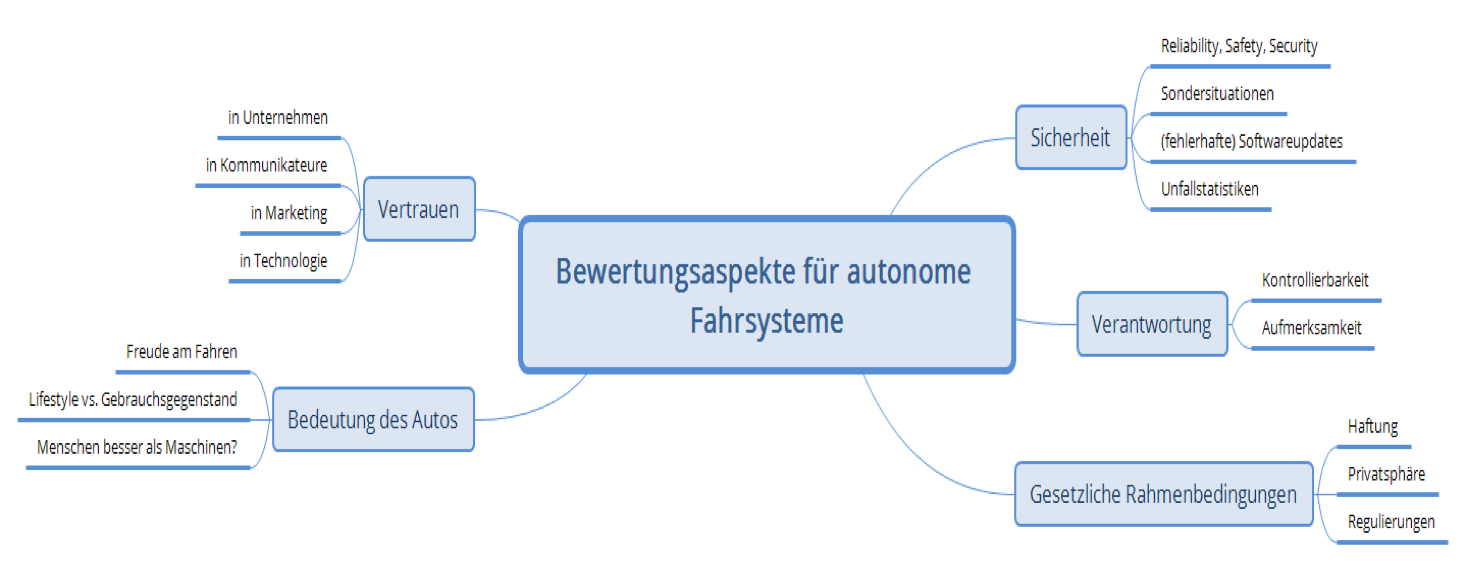
\includegraphics[width=13cm]{Webanlayse.png}
  \caption{Übersicht über die Kategorien aus der Webanalyse}
  \label{fig:gehirn-beim-arbeiten-anschalten1}
\end{figure}

Um im Interview differenzierte Aussagen zu gewinnen, wurden diese Oberkategorien als inhaltlicher Überbau übernommen und textuell angepasst. Der finale Stand der Kategorien sah nach dem ersten deduktiven Schritt wie folgt aus: \emph{Anforderungen},  \emph{Gefahren und Probleme}, \emph{Vertrauen}, \emph{Vorannahmen}, \emph{Informiertheit}, \emph{Fahraufgaben behalten/abgeben}, \emph{Kriterien eines guten Beifahrers} und \emph{Überforderung} sowie \emph{Erfahrung}. Um diese Kategorien bildeten sich die Rahmenfragen des Interviewleitfadens. Zum Vergleich wurde für die Interviewstudie noch die etablierte Technologie von Fahrassistensysteme dazu genommen. Dadurch sollten Unterschiede zwischen einer bereits etablierten Technologie und einer, die aktuell die Gesellschaft verändert, beleuchtet werden können.

Bei den Kategorien wurde jeweils zwischen autonomen Fahren und Fahrassistenzsysteme unterschieden. Während der Auswertung der Interviews wurde jedoch ersichtlich, dass dezidierte Aussagen zu bestimmten Themenbereichen nicht möglich waren. Vor allem der Vergleich zwischen autonomen Fahren und Fahrassistenzsysteme war mittels des gesammelten Materials nicht möglich. Dies führte dazu, dass anhand des Interviewmaterials die finalen Kategorien der beiden Technologien zusammengefasst und die übrigen Kategorien geschärft werden mussten. %TODO: ich verstehe den letzten Satz nicht wirklich. Kann Josh da noch einmal drüber gehen?

Insgesamt sind Kommentare aus den Interviews extrahiert worden und bilden den Korpus des Kategoriensystems.In weiterern Analysedurchläufen wurde geprüft, ob sich die einzelen Kommentare überscheidungsfrei den Kategorien zuordnen lassen.

Das finale Kategoriensystem umfasste die Oberkategorien \emph{Vorannahmen der Befragten}, \emph{Kenntnisstand der Befragten} und \emph{Kriterien eines guten Beifahrers}. Die restlichen Oberkategorien lauten \emph{Anforderungen an Fahrassistenzsysteme}, \emph{Gefahren und Probleme}, \emph{Vertrauen} \emph{Fahraufgaben abgeben} und \emph{Fahraufgaben behalten}. Die Bedeutung der einzelnen Kategorien lässt sich an der Namensgebung ablesen. Weitere Unterkategorien sind induktiv aus dem Datenmaterial erschlossen worden und werden im Ergebnissteil genauer beleuchtet.

Das finale System aus Oberkategorien sieht wie folgt aus:

\begin{figure}[htp]
  \centering
  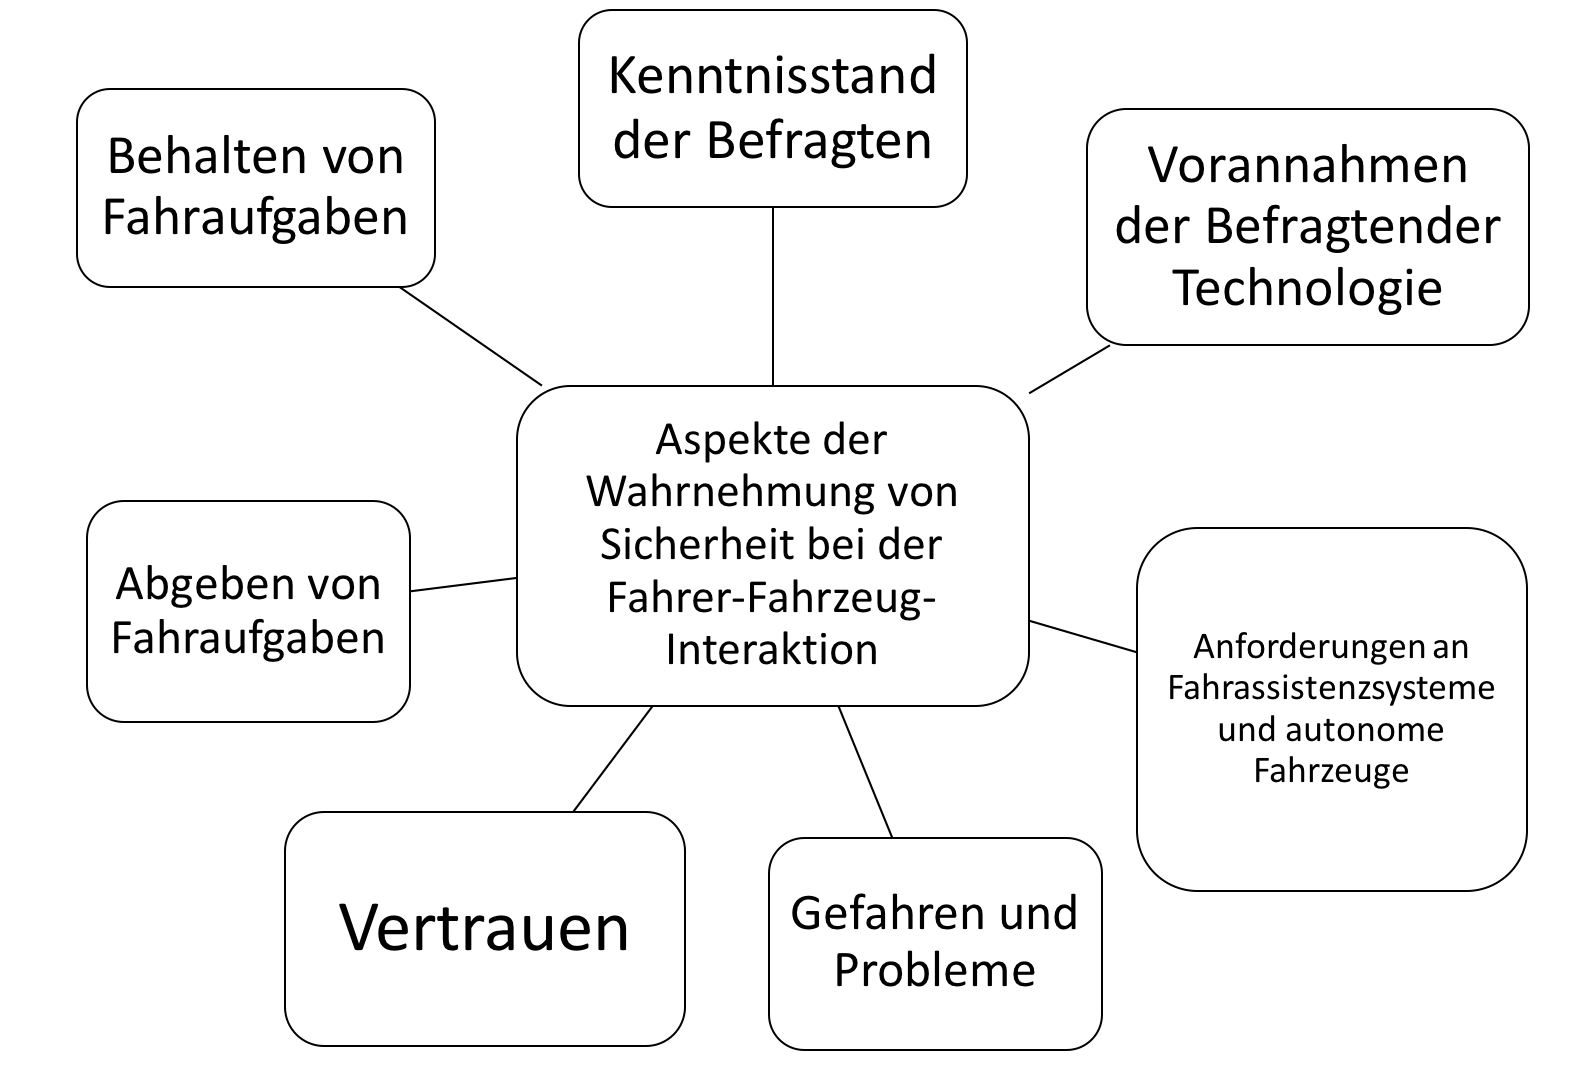
\includegraphics[width=13cm]{Kategoriensystem.png}
  \caption{Die Oberkategorien nach dem letzten deduktiven Schritt}
  \label{fig:gehirn-beim-arbeiten-anschalten2}
\end{figure}

\clearpage
\section{Ergebnisse}
Im Folgenden werden die Ergebnisse der Studie vorgestellt. Da die Bewertung der Sicherheit vor den jeweilig persönlichen Hintergründen der Befragten zu betrachten sind, werden zunächst einige Vorinformationen über die Befragten betrachtet.

% \subsection*{Personendaten}
% Unter den sechs Befragten waren fünf Männer und eine Frau. Alle Befragten waren zwischen 23 und 29 Jahren alt, mit einem mittleren Alter von 25 Jahren, Median von 24 Jahren. Die Befragten hatten ihren Führerschein seit mindestens fünf Jahren. Der erfahrenste Fahrer war bereits 12 Jahre im Besitz der Fahrerlaubnis.
%
% Die Hälfte der Befragten war zum Zeitpunkt der Erhebung im Besitz eines eigenen PKW, die anderen 38\,\% nutzten geteilte Fahrzeuge, z.\,B. der Eltern oder Car-Sharing Angebote.
%
% Familienstand und Einkommen wurden nicht erhoben, die Mehrzahl der Befragten ist jedoch als Student tätig.

\subsection{Kenntnisstand der Befragten}
Der Wissensstand der Befragten zum Thema Fahrassistenzsysteme und autonomes Fahren war zum Zeitpunkt der Befragung gemischt. Auch, wenn die Mehrheit der Befragten selbst noch keine praktische Erfahrung mit entsprechenden Systemen gemacht hat, waren die Befragten durch die Presse (B03, Z. 98; B04, Z. 113) und durch allgemeines Vorwissen (B01, Z. 74ff) zumindest grundsätzlich über das Thema informiert.

Detail- und Anwendungswissen war bei der Hälfte der Befragten nicht vorhanden (B02, Z.44; B03, Z. 30, B05.3, Z. 24), die restlichen Befragten können  zu einzelnen Assistenzsystemen aus eigenen Erfahrungen berichten (B01, Z. 34, 38; B04 Z. 32-37; B06.2, Z. 12).

Konkrete Kenntnisse haben die Kandidaten zu folgenden Assistenzsystemen:
\begin{itemize}
  \item Bremsassistent (B01, Z. 34; B04, Z. 29)
  \item Verkehrszeichenerkennung (B01, Z. 38)
  \item Spurhalteassistent (B01, Z. 38; B04, Z. 29)
  \item Abstandshalter (B04, Z. 29)
  \item Tempomat (B04, Z. 29)
  \item Einparkhilfen (B03, Z. 32; B06.2, Z. 12)
\end{itemize}

Kandidaten, die keine Erfahrungen mit Fahrassistenzsystemen oder autonomen Fahrzeugen machen konnten, nannten dafür folgende Gründe:
\begin{itemize}
  \item Kein Zugang zu entsprechenden Fahrzeugen (B03, Z. 32, 78; B06, Z. 12)
  \item Eigener PKW nicht mit Fahrassistenzsystemen ausgestattet (B02, Z. 46)
  \item Fahrassistenzsysteme kein Kaufkriterium (B06.2, Z. 18)
\end{itemize}


\subsection{Vorannahmen der Befragten}
Einige Äußerungen der Kandidaten ließen auf Vorannahmen bezüglich autonomem und unterstütztem Fahren schließen. Im Folgenden sind diese Vorannahmen aufgelistet und erläutert. Diese Vorannahmen dienen als Kontext zur besseren Einordnung der Ergebnisse.
\subsubsection*{Berichterstattung in der Presse}
Ein Befragter äußerte, dass er von einer negativen Färbung der Berichterstattung in den Medien über das Thema autonomes/assistiertes Fahren ausgeht.

\begin{quote}
  Meistens kommt ja auch nur das Negative dann in die Presse und nicht das Auto fährt jetzt seit 100.000 Km autonom erfolgreich. Nein, da kommt was, wenn es einen übergebretzelt hat. (B04, Z. 113)
\end{quote}

\subsubsection*{Überlegenheit von Technik}
Es gab weiterhin Äußerungen der Befragten, die nahelegen, dass Grundannahmen darüber vorherrschen, ob und wenn ja in welchen Fällen die Technologie besser ist als der Mensch.

\begin{quote}
  Wenn [...] wirklich alle Autos miteinander vernetzt wären, dann hättest du wahrscheinlich keinen Stau mehr, weil du einsteigst, dein Ziel eingibst, dann rechnet das das wahrscheinlich gut raus, es würde wahrscheinlich sehr viele Probleme lösen, [...] die Autos sparen super viel Sprit, scheiden weniger Abgase aus. Wahrscheinlich ist alles viel flüssiger, du bist viel schneller unterwegs. (B04, Z. 73)
\end{quote}

Äußerungen in diesem Zusammenhang sprachen Fahrassistenzsystemen bzw. autonomen Fahrzeugen zu, dass sie

\begin{itemize}
  \item Besser als Menschen fahren (B01, Z. 96; B04, Z. 69)
  \item Zuverlässigere Teilnehmer im Straßenverkehr sind (B04, Z. 73)
  \item Stau reduzieren (B04, Z. 73)
  \item Besser einparken als Menschen (B05.2, Z. 31)
\end{itemize}

\subsubsection*{Sicherheit der Technologie}
Die Befragten waren sich nicht einig darüber, inwiefern die Technologie hinter autonomem Fahren bzw. Fahrassistenzsystemen sicher ist. Auf der einen Seite wurden die Systeme als \glqq zum größten Teil sicher\grqq{} (B01, Z. 62) bezeichnet. Auf der anderen Seite wurden von vier der sechs Kandidaten Äußerungen getroffen, die die allgemeine Sicherheit der Systeme in Frage stellen (B01, Z. 44; B02, Z. 34; B03, Z. 50, 72, 98; B06.3, Z. 18, 28).

\begin{quote}
  Obwohl ich da glaube ich noch etwas misstrauisch bin, ob das immer so gut funktioniert. (B02, Z. 34)
\end{quote}

Darüber hinaus äußerte ein Befragter starke Bedenken, ob absolute Sicherheit überhaupt gewährleistet werden kann:

\begin{quote}
  Vollendete - also völlige Sicherheit gibt es nur, wenn du dich im Bunker einschließt. (B03, Z. 56)
\end{quote}

\subsubsection*{Vertrauen in Fahrassistenzsysteme und autonome Fahrzeuge}
Zwei der Befragten äußerten sich zu ihrer grundsätzlichen Einstellung gegenüber Fahrassistenzsystemen. Beide haben Vertrauen in Fahrassistenzsysteme, schränken diese Aussage aber auch ein (B01, Z. 54; B04, Z. 63).

\begin{quote}
  Obwohl ich den Systemen schon sehr vertraue. Also ist jetzt nicht so, dass ich da komplett gegen bin oder so. (B01, Z. 54)
\end{quote}

Die übrigen Befragten haben keine Aussagen getroffen, die eine eindeutige Aussage zu grundsätzlichem Miss- oder Vertrauen zulassen.

\subsubsection*{Hohe Anschaffungskosten der Technologie}
Eine weitere Vorannahme, die bei zwei Kandidaten festgestellt werden konnte, ist die Annahme, dass eine neue Technologie wie Fahrassistenzsysteme oder autonome Fahrzeuge in der Anschaffung besonders teuer sind. (B02, Z. 48; B03, Z. 102)

\begin{quote}
  Da die Autos dann wahrscheinlich genauso viel, wenn nicht sogar noch mehr wie ein jetziges, normales Auto kosten sind die für mich dann nicht rentabel. (B03, Z. 102)
\end{quote}


\subsection{Anforderugnen an Fahrassistenzsysteme und autonome Fahrzeuge}
In den Gesprächen nannten die Befragten mehrere Gruppen von Anforderungen, die Fahrassistenzsysteme und autonome Fahrzeuge erfüllen sollen. Diese werden im Folgenden erörtert.

\subsubsection*{Überlegenheit gegenüber dem Menschen}
Zwei der Befragten nannten als Anforderung, dass Fahrassistenzsysteme und insbesondere autonome Fahrzeuge normalen menschlichen Autofahrern in Punkto Fahren mindestens gleichwertig, besser aber überlegen sein müssen (B03, Z. 94; B04, Z. 105).

\begin{quote}
  sie müssen halt mindestens genausogut, eher sogar noch besser als ein jetziger, normaler Autofahrer sein
\end{quote}

Die Befragten schließen hier auch über die reine Fahrsicherheit hinausgehende Aspekte ein. Explizit genannt wird zwar die Reaktionsfähigkeit (B03, Z. 94) und Wahrnehmung des Umfeldes (B04, Z. 105) aber es ist auch die Rede von \glqq der gesamten Fähigkeit, Auto zu fahren im Straßenverkehr\grqq{} (B03, Z. 94).

\subsubsection*{Zuverlässiges Erkennen von Situationen}
Dass Fahrassistenzsysteme und autonome Fahrzeuge über die Fähigkeit verfügen, Verkehrssituationen und -teilnehmer insbesonbdere auch unter außergewöhnlichen Umständen korrekt zu erfassen, war für einen der Befragten eine konkrete Anforderung (B02, Z. 70, 114).

\begin{quote}
  Also die müssen flexibel genug sein, alle Problematiken zu erkennen. Also zum Beispiel [...] ein Fahrrad mit [...] zwei Hinterrädern oder zwei Vorderrädern, eine andere Form, wird anders erkannt… [...] das System muss flexibel genug sein das zu erkennen, wenn auch mal ein Gerät ein bisschen anders aussieht als sonst. (B02, Z. 70)
\end{quote}

\subsubsection*{Vermitteln eines Sicherheitsgefühls}
Zwei Befragte nannten als Anforderung, dass Fahrassistenzsysteme und autonome Fahrzeuge dem Fahrer und auch den anderen Verkehrsteilnehmern ein Gefühl der Sicherheit vermitteln sollten (B03, Z. 78; B04 Z. 39, 111). In diesem Zusammenhang klingt an, dass solche Systeme ihre Intention oft nicht klar machen; ein Befragter beschwert sich: \glqq kein Mensch fährt halt so\grqq{} (B04, Z. 39).

\subsubsection*{Möglichkeit für menschliche Intervention}
Eine weitere von mehreren Befragten angeführte Anforderung war, dass der Mensch stets noch die Chance hat, manuell das Fahrgeschehen zu beeinflussen (B02, Z. 82, 106; B06.3, Z. 36). Insbesondere war den Befragten dies wichtig, für den Fall, dass \glqq das Fahrzeug Dinge macht, die man nicht möchte\grqq{} (B02, Z. 82).

\begin{quote}
  Was ich mir vorstellen könnte, dass man trotzdem noch eingreifen kann. (B06.3, Z. 36)
\end{quote}

Allen Befragten ging es hierbei in letzter Konsequenz hauptsächlich um das Vermeiden von Unfällen.

\subsubsection*{Geringe Ausfallquote}
Ein einzelner Befragter nannte als Anforderung, dass Fahrassistenzsysteme und autonome Fahrzeuge eine möglichst gerine Ausfallquote haben sollten.

\begin{quote}
  Oder besser gesagt geringe Fehlerrate, also keine Ausfall - geringe Ausfallquote. (B03, Z.52)
\end{quote}

\subsubsection*{Unabhängige Prüfstellen}
Einer der Befragten nannte die Anforderung, dass Systeme von unabhängigen, spezialisierten Prüfstellen abgenommen werden sollen. Als Vergleich wird der TÜV genannt.

\begin{quote}
  Ich finde, es sollte halt einfach sowas in Deutschland den TÜV, der sich damit dann hoffentlich auch auskennt sowas prüfen und testen [...]. (B04, Z. 107)
\end{quote}

\subsubsection*{Klar beschriebener Funktionsumfang}
Eine weitere genannte Anforderung ist ein klar beschriebener Funktionsumfang. Das System solle \glqq das tun, was draufsteht\grqq{}. (B03, Z. 52)


\subsection{Gefahren und Probleme}
In der Befragung wurde erhoben, welche möglichen Gefahren und Probleme die Kandidaten im Kontext von Fahrassistenzsystemen und autonomen Fahrzeugen wahrnehmen. Im Folgenden sind die genannten Punkte gelistet.

\subsubsection*{Wartung}
Ein Befragter äußerte Bedenken zu Gefahren, die durch mangelnde Wartung von autonomen oder unterstützenden Fahrsystemen ausgehen. Der Befragte äußerte, dass seiner Einschätzung nach viele Menschen ihre Fahrzeuge generell schon stark vernachlässigen würden. Er sieht ein Gefahrenpotenzial, falls entsprechende Systeme nicht ordnungsgemäß instandgehalten werden. Der Kandidat vergleicht das Gefahrenpotenzial mit Risiken, die durch die TÜV-Kontrollen abgedeckt werden und kommt zu der Einschätzung, dass sich das Niveau des Risikos auf der gleichen Stufe befindet (B04, Z. 105).

\subsubsection*{Rechtliche Bedenken}
Die Hälfte der Befragten äußerte Bedenken, was rechtliche Fragen im Bezug auf Fahrassistenzsysteme und autonome Fahrzeuge angeht. Ganz allgemein formulierte es einer der Befragten: \glqq Viel Rechtliches. Noch. Weil viel da nicht geklärt ist und ich weiß nicht, wie schnell sich das entwickelt. Aber da muss man nachziehen\grqq{} (B04, Z. 105).

Ein weiterer Aspekt, der genannt wurde, ist der Datenschutz:

\begin{quote}
  Dass [...] Dritte wissen, wo ich mich gerade befinde und viele Zusatzinformationen über mein Auto haben, das würde mich stören. (B02, Z.76)
\end{quote}

Auf die Frage nach der Schuld im Falle eines Unfalls waren die Befragten unterschiedlicher Meinung. Als mögliche Schuldige bei einem Unfall nannten die Befragten:
\begin{itemize}
  \item Den Hersteller (B02, Z. 78)
  \item Den Programmierer der Software, falls die Software fehlerhaft war (B03, Z. 64, 100)
  \item Den Ingenieur des Fahrzeugs, falls die Konstruktion des Fahrzeugs fehlerhaft war (B03, Z. 100)
  \item Dem Fahrer, falls er seine Aufsichtsverantwortung bei einem Fahrassistenzsystem missachtet hat (B01, Z. 94; B04, Z. 75)
  \item Nicht dem Fahrer, falls das Fahrzeug autonom fährt (B04, Z. 75)
  \item Niemandem (B03, Z. 64, 100)
\end{itemize}

Die Befragten geben hier kein einheitliches Meinungsbild. Zu einer sehr differenzierten Einschätzung kommt einer der Befragten auf die Frage nach der Unfallschuld bei einem verunfallten autonomen Fahrzeug:

\begin{quote}
  Hm. Ich weiß nicht, wie - also nicht der Fahrer, meiner Meinung nach - aber ich weiß nicht, wie die Abgrenzung dann im Bereich ist von den verschiedenen Herstellern. Weil ich finde, dann kommt es stark darauf an, was versagt hat: War es Software, war es irgend ein Sensor... Warum, wenn ein Sensor? Liegt es daran, dass der kaputt war und der Fahrer sich nicht darum gekümmert hat, dann ist es doch wieder der Fahrer. Das sind halt viel zu viele kleine Faktoren als dass man das pauschalisieren könnte. (B04, Z. 115)
\end{quote}

\subsubsection*{Moralische Fragen}
Ebenfalls angeführt wurde die Problematik der moralischen Fragen, die im Kontext von autonomen Fahrzeugen und Fahrassistenzsystemen aufkommen. Ein Befragter nannte konkret das Beispiel von unvermeidlichen Unfällen, wo das Fahrzeug selbst eine Entscheidung zwischen zwei Übeln treffen muss (B03, Z. 90).

\begin{quote}
  Wenn ein Unfall unvermeidbar ist, was macht das autonome Auto. Ja das ist die Moral. (B03, Z. 90)
\end{quote}

\subsubsection*{Überhöhtes Vertrauen in Technik}
Beinahe alle Befragten äußerten, dass Fahrer, die sich zu sehr auf ihr Fahrzeug verlassen ein Risiko darstellen (B01, Z. 50; B02, Z. 66; B03, Z. 50; B04, Z. 57; B06.2, Z. 36).

\begin{quote}
  Ich glaub es kann gefährlich sein, wenn man sich zu sehr darauf verlässt und bei diesen Leuchten im Außenspiegel, die aufleuchten, wenn man überholt wird oder wenn ein Auto von hinten kommt, das man sich nur noch darauf verlässt und nicht mehr selber guckt. Und es kann immer sein das es mal nicht funktioniert und die Leute sich zu sehr darauf verlassen [...]. (B06.2, Z. 36)
\end{quote}

Darüber, wie sich das überhöhte Vertrauen konkret auswirken kann, hatten die Befragten unterschiedliche Einschätzungen:
\begin{itemize}
  \item Erhöhte Unfallgefahr (B01, Z. 50; B02, Z. 66; B03, Z. 50)
  \item Einschränkung/Verwirrung des Fahrers (B01, Z. 50)
  \item Erhöhte Wahrscheinlichkeit von Fahrfehlern (B03, Z. 50)
  \item Verleiten zu Unachtsamkeit (B04, Z.57)
\end{itemize}

\subsubsection*{Unachtsamkeit des Fahrers}
Als weitere Gefahr sehen die Befragten, dass Fahrer durch Fahrassistenzsysteme unachtsam im Straßenverkehr werden. Die Unachtsamkeit muss aber nicht notwendigerweise durch ein überhöhtes Vertrauen in die Assistenzsysteme eines Fahrzeugs bedingt sein, sondern kann auch grundsätzliche Unaufmerksamkeit des Fahrers bedeuten. Besonders hervorgehoben werden außergewöhnliche Situationen, in denen der Fahrer eingreifen müsste, es aber aufgrund von Unachtsamkeit nicht tut (B04, Z. 57; B05.2, Z. 25).

Weiterhin genannt werden Assistenzsysteme, die aktiv vom Fahrer beachtet werden müssen, wie z.\,B. Toter-Winkel-Warner. Diese benötigen die Aufmerksamkeit des Fahrers, um wirksam zu sein (B04, Z. 65).

\subsubsection*{Cyberattacken}
Zwei der Befragten sahen in der Tatsache, dass Fahrzeuge mit Fahrassistenzsystemen oder autonomen Fahrfunktionen häufig mit Netzwerk-Technolgien ausgestattet sind ein Gefahrenpotenzial für Cyberattacken. Explizit genannt wird die \glqq Ausnahmegefahr von Anschlägen\grqq{} (B03, Z.62) auf Grund der erhöhten Angreifbarkeit von zentral gesteuerten Systemen (B01, Z. 66; B03, Z. 62, 92).

Neben der diffusen Gefahr des Hackerangriffs nannte ein Befragter konkrete Gefährdungsszenarien, die von Cyberattacken auf Fahrzeuge ausgehen: (B03, Z. 92)
\begin{itemize}
  \item Absichtliches Verursachen von Unfällen
  \item Entführen von Fahrzeugen aus der Ferne
\end{itemize}

\subsubsection*{Unzuverlässigkeit anderer (menschlicher) Verkehrsteilnehmer}
Weiterhin als Gefahr identifiziert werden die Unzulänglichkeiten nicht des autonomen bzw. unterstützen Autoverkehrs, sondern solche, die durch dritte Verkehrsteilnehmer entstehen (B01, Z. 52-60, 88-92; B05.3 Z. 25).

\begin{quote}
  Ich glaube, dass sehr viele andere Autofahrer das Problem sind, und halt keine Standardsituationen wie Baustellen und Staus oder sowas. (B01, Z. 52)
\end{quote}

Hervorgehoben wurden von einer Person Fahrradfahrer, die sich über Verkehrsregeln hinwegsetzen (B01, Z. 60).

\subsubsection*{Unerwartetes Verhalten des Autos}
Befragte schilderten außerdem, wie unerwartetes Verhalten ihres von einem Assistenzsystem geleiteten oder autonom fahrenden Vehikels Gefahre oder Probleme darstellen könnten (B01, Z. 50; B02, Z. 106; B05.2, Z. 25; B06.2, Z. 42).

\begin{quote}
  Gerade wenn man in ein Parkhaus reinfährt, da macht der schon mal gern ne Vollbremsung vor so ner Schranke. (B01, Z. 50)
\end{quote}

Folgende Situationen wurden in diesem Zusammenhang von den Befragten genannt:
\begin{itemize}
  \item Aktiver Spurhalteassistent vom Fahrer vergessen: Das Auto lenkt gegen und \glqq überschreibt\grqq{} menschliche Aktion (B01, Z. 50)
  \item Zufahren auf Schranke (z.\,B.: im Parkhaus): Das Auto bremst stark und unerwartet (B01, Z. 50)
  \item Technischer Aussetzer: Der Fahrer ist nicht darauf vorbereitet, dass das Fahrassistenzsystem ausfällt (B05.2, Z. 25)
  \item Abbiegen des Autos: Von außen als Fahrradfahrer möglicherweise nicht erkennbar (B06.2, Z.42)
\end{itemize}

\subsubsection*{Erkennung von Situationen}
Vier der Teilnehmer nannten als mögliche Gefahr, dass Verkehrssituationen von den Fahrzeugen nicht korrekt erkannt werden.

\begin{quote}
  Wenn man zum Beispiel mit dem Spurhalteassistenten in die Baustelle reinfährt, erkennt der nicht, dass weiße Streifen aufhören und gelbe da sind, und versucht dann mitzulenken, das wird dann schwierig. (B01, Z. 44)
\end{quote}

Folgende Situationen wurden hierbei von den Befragten genannt:
\begin{itemize}
  \item Baustellen, bzw. der Wechsel von weißen zu gelben Fahrbahnmarkierungen (B01, Z. 44)
  \item Erkennung von Fahrzeugen in besonderen Lichtsituationen (B01, Z. 88)
  \item Parkhilfen, die Entfernungen falsch bemessen (B02, Z. 66)
  \item Fahrradfahrer, sowohl als false-positive (B04, Z. 67) als auch als false-negative (B04, Z. 65)
\end{itemize}

\subsubsection*{Ausfall der Sensorik}
Weiterhin wurde als potenzielle Gefahr der Ausfall der von den Assistenzsystemen oder autonomen Fahrzeugen benötigten Sensorik genannt (B02, Z. 66, 106; B06.3, Z. 18, 28).

\begin{quote}
  Also dass die Sensorik zum Beispiel bei einem Abstandshalter spinnt, kaputtgeht, und dann nicht mehr funktioniert. (B02, Z. 66)
\end{quote}

In diesem Zusammenhang wurden von einer Person mehrfach Vergleiche zu Alltagstechnologien wie Handy oder Laptop und deren in ihrer Erfahrung hohen Ausfallquote gezogen (B06.3, Z. 18, 28).


\subsection{Vertrauen}
Während der Interviews äußerten sich mehrere Befragten in Bezug auf Vertrauen. Diese Äußerungen werden hier strukturiert wiedergegeben.

\subsubsection*{Institutionen in Deutschland}
Ein Befrater äußerte, dass seiner Einschätzung nach insbesondere in Deutschland ausschließlich funktionierende Fahrzeuge für den Straßenverkehr zugelassen sind:

\begin{quote}
  Das wird - vor allem, gehen wir jetzt mal wir leben ja in Deutschland, das wird ausgiebig getestet vermutlich. Ich denke, das wird funktionieren, sonst würde das nicht einfach so auf die Straße gelassen werden. (B04, Z. 51)
\end{quote}

\subsubsection*{Historie als Vertrauensfaktor}
Für das Vertrauen zu Automobilherstellern und deren Fahrzeuge war für einen der Befragten das Verhalten dieses Unternehmens in der Vergangenheit besonders wichtig (B03, Z. 48, 88).

\begin{quote}
  Ich wüsste jetzt nicht, dass irgendwer da grob Unfähigkeiten gibt oder gezeigt hat, dass er grob unfähig in dem Bereich ist. (B03, Z. 88)
\end{quote}

Explizit genannt wurde in diesem Zusammenhang auch der Dieselskandal (B03, Z. 48).

\subsubsection*{Vertrauen in Automarken}
Auf die Frage nach Miss- oder Vertrauen in einzelne Automarken gaben die Interviewpartner verschiedene Antworten.

Einer der Befragten nannte Tesla als vertrauenswürdige Automarke und begründete diese Entscheidung mit langen unfallfreien Fahrzeiten und einer von ihm positiv Bewerteten Krisenkommunikation des Geschäftsführers von Tesla. Als Vergleichsobjekt zog der Befragte Ford heran; Er würde Tesla mehr vertrauen als zum Beispiel Ford (B01, 82ff).

Weiterhin wurden VW und Audi als nicht vertrauenswürdige Automarken genannt, Grund hierfür sei der Dieselskandal. (B03, Z.42; B05.2, Z. 15) Einer der Befragten ging zusätzlich ins Detail: Obwohl er den Unternehmen grundsätzlich gute Intentionen unterstellt, herrscht Misstrauen; Sowohl was die Qualität der Produkte in Punkto Fehlerfreiheit angeht, als auch was die Selbstdarstellung des Unternehmens in Marketing und Öffentlichkeitsarbeit angeht. Abwiegelnd äußert der Befragte außerdem, dass die Großunternehmen auch monetäre Interessen verfolgen (B03, Z. 42ff).

Von allgemein guten Erfahrungen mit den Automarken VW (mit Einschränkung des Abgasskandals), BMW, Audi, Skoda und Volvo berichtet ein weiterer Befragter (B05.2, Z.15). Auf Nachfrage nennt er folgende Kriterien für seine Bewertung von Automarken (B05.2, Z. 17):
\begin{itemize}
  \item Fahrkomfort
  \item Sicherheit
  \item Fahrspaß
  \item Erfüllen des gewünschten Funktionsumfangs
\end{itemize}

Davon abgesehen gab es eine wesentlich abstraktere Einschätzung: Einer der Befragten beurteilte die Qualität der Fahrassistenzsysteme als \glqq auf dem ungefähr gleichen Niveau\grqq{} (B04, Z. 49) fügte aber im weiteren Verlauf des Interviews hinzu:

\begin{quote}
  Ja das auf sone Automarkengeschichte herunterzupressen find ich schwierig. In Automarken geht auch immer viel persönlicher Geschmack und sowas ein. [...] Ich weiß auch nicht ob jeder Autohersteller das komplett selber entwickelt, deshalb ist das schwierig, das mit der Marke in Verbindung zu setzen [...]. (B04, Z. 103)
\end{quote}

\subsubsection*{Vertrauen durch Erfahrungswerte}
Mehrere Befragte vermissen persönliche Erfahrungen mit Fahrassistenzsystemen oder autonomen Fahrzeugen, um sich eine bessere Meinung bilden zu können. Hierbei ging es den Befragten um eine Befriedigung der persönlichen Neugierde (B04, Z. 91ff), Vertrauensbildung (B05.3 Z.22; B06.3, Z. 24ff) oder allgemeine Erweiterung des Erfahrungsschatzes (B06.2, Z. 32).

\begin{quote}
  Ich glaube es würde helfen, wenn die Sachen mehr Präsenz im Alltag bekommen würde, man bekommt hier einfach nichts mit bzw. ich kriege nichts mit. Wenn es einfach ein bisschen präsenter werden würde. Dann sieht man das es funktioniert und es gut funktioniert. (B06.3, Z. 24)
\end{quote}

\subsubsection*{Vertrauen durch Transparenz}
Ein weiterer Aspekt, der für Vertrauen genannt wurde, war Transparenz. Dies hieß für die Befragten Unterschiedliches:
\begin{itemize}
  \item Aufbereitete Rohdaten von Tests (B02, Z. 60ff)
  \item Aufrichtige Kommunikation über Produkte (\glqq Vernünftig produzieren und das abliefern, was sie auch draufschreiben\grqq{} (B03, Z. 84))
  \item Offene Kommunikation über Wissensstand und Fortschritt des Unternehmens (B04, Z. 99)
  \item Angemessene kommunikative Lösungen für Restrisiken (B04, Z. 105)
\end{itemize}

\subsection{Abgeben von Fahraufgaben}
In den Gesprächen wurden Situationen erfragt, in denen die Befragten gerne Fahraufgaben abgeben würden oder bereits auf Fahraufgaben verzichten. Weiterhin wurden Argumente für und gegen das Abgeben dieser Fahraufgaben gesammelt.

\subsubsection*{Stadtstrecken}
Bereitschaft zum abgeben von Fahraufgaben herrscht bei zwei der Befragten in Städten (B02, Z. 20; B04, Z. 95), einer der beiden hebt fremde bzw. unbekannte Städte hervor und nennt Überforderung mit Ampeln und Abbiegerspuren als Begründung.

\begin{quote}
  Und in unbekannten Städten, also in Städten wo ich nicht weiß, wie man normalerweise fährt. Da bin ich schnell überfordert mit Ampeln, Abbiegerspuren etc. (B04, Z. 95)
\end{quote}

\subsubsection*{Alkoholkonsum}
Einer der Befragten nannte als Situation, in der er das Fahren vermeidet den Zustand der Trunkenheit oder des Verkatert-Seins.

\begin{quote}
  Wenn ich verkatert bin. Dann fahr ich danach eigentlich sehr ungern Auto. (B03, Z. 14)
\end{quote}

Es kann mit einiger Wahrscheinlichkeit davon ausgegangen werden, dass dies für die übrigen Befragten so selbstverständlich war, dass sie es nicht gesondert erwähnt haben.

\subsubsection*{Bremsen}
Ein Befragter äußerte, dass er gerne das Bremsen an einen Bremsassistenten abgeben würde, um Auffahrunfälle zu vermeiden.

\begin{quote}
  Also ich kann mir vorstellen, zum Beispiel ein Bremssystem. [...] Ein Abstandsmesser der eingreift, wenn du gedanklich kurz abwesend bist. Damit können Auffahrunfälle nicht mehr passieren. (B05.1, Z. 16)
\end{quote}

\subsubsection*{Autobahnfahrten}
Mehrfach genannt wurden lange Fahrten auf der Autobahn, bei denen Befragte gerne Teile des Fahrens an Assistenzsysteme abgeben würden (B01, Z. 38; B02, Z. 28ff; B03, Z. 22, 62; B04, Z. 23, 37, 95; B05.1, Z. 10; B06.1, Z. 20; B06.2, Z. 58; B06.3, Z. 10).

Folgende Fahraufgaben sollen bei Autobahnfahrten abgegeben werden:
\begin{itemize}
  \item Abstand halten (B02, Z. 28; B04, Z. 23)
  \item Geschwindigkeit halten (B02, Z. 28; B06.1, Z. 20)
  \item Stop-and-Go im Stau (B03, Z. 62; B04, Z. 23; B05.1, Z. 10B06.1 Z. 20)
  \item Bilden einer Rettungsgasse (B06.2 Z. 58)
\end{itemize}

Folgende Gründe werden zum Abgeben der Fahraufgaben bei Autobahnfarten genannt:
\begin{itemize}
  \item Konzentration über lange Zeit (B02, Z. 8; B06.3, Z. 10)
  \item Ermüdung auf langen Strecken (B04, Z. 37)
  \item Fahraufgaben nervenaufreibend (B03, Z. 62; B05.1, Z. 10; B06.1, Z. 20)
  \item Könnte Stau reduzieren (B04, Z. 23)
  \item Menschliche Autofahrer nicht fähig genug (B06.2, Z. 58)
\end{itemize}

\subsubsection*{Einparken}
Ein weiterer Aspekt, der in einem Gespräch genannt wurde ist das Einparken.

\begin{quote}
  Ja, also parken könnte ich mir auch vorstellen, dass mir das abgenommen wird. (B02, Z. 34)
\end{quote}

Der Befragte beschrieb Parken als \glqq Situation, die ich sehr schlecht finde\grqq{} (B02, Z. 20) und wünscht sich entsprechend ein System, das ihn bei dieser Fahraufgabe unterstützt.

\subsubsection*{Negative Grundhaltung zum Autofahren}
Einer der Befragten nannte als möglichen Grund für das Abgeben von Fahraufgaben, dass Personen möglicherweise grundsätzlich nicht gerne mit dem Auto fahren (B03, Z.22).

\subsubsection*{Körperliche Einschränkungen}
Körperliche Einschränkungen können auch ein Grund dafür sein, dass Personen Fahraugaben abgeben wollen. So nannten Befragte das Alter des Fahrers oder eingeschränktes Sehvermögen (B03, Z. 22). Darüber hinaus äußerte ein Interviewpartner, dass er sich nach starker körperlicher Anstrengung manchmal wünscht, das manuelle Schalten aufzugeben und seinem Fahrzeug zu überlassen (B01, Z. 18):

\begin{quote}
  Also, gerade nach nem Marathon oder Triathlon sind die Beine manchmal etwas schwer. Da wünscht man sich dann doch ne Automatik.
\end{quote}


\subsection{Behalten von Fahraufgaben}
Ebenfalls erhoben wurde, welche Argumente es für Autofahrer gibt, Fahraugaben nicht abzugeben sondern zu behalten.

\subsubsection*{Mangelndes Vertrauen in Technik}
Einer der Befragten nannte mangelndes Vertrauen als möglichen Grund für Fahrer, Fahraufgaben lieber selbst zu erledigen. Dabei bezieht er Vertrauen sowohl auf die Qualität des Systems als auch auf die Sicherheit (B04, Z. 25, 39).

\begin{quote}
  Weil ich glaube, die meisten haben nicht so das Vertrauen und würden das nicht gerne abgeben wollen. Und denken auch, sie können es besser [...]. (B04, Z. 25)
\end{quote}

\subsubsection*{Unwissen über Möglichkeiten}
Einer der Befragten antwortete auf die Fragen danach, ob er Teile des Fahrens abgeben wollen würde mit:

\begin{quote}
  Ne. Also. Ich wüsste jetzt nicht, welche. (B03, Z. 20)
\end{quote}

\subsubsection*{Selbstbestimmtheit}
Ein weiteres Argument dafür, Fahraufgaben zu behalten scheint die Selbstbestimmtheit des Autofahrers zu sein. Hierbei spielt zum Beispiel das bewusste Übertreten von Geschwindigkeitsbegrenzungen eine Rolle, die sonst vom Assistenten oder autonomen Fahrzeug penibel eingehalten würden (B02, Z. 36; B04, Z. 37).

\subsubsection*{Freude am Autofahren}
Mehrere der Befragten nannten Fahrspaß bzw. freude am Autofahren als Hindernis dafür, Fahrassistenzsysteme oder autonome Fahrzeuge zu verwenden (B01, Z. 18, 30; B02, Z. 36; B04, Z. 95; B06.1, Z. 22).

Als besonderer Spaßfaktor wurde mehrfach schnelles Autofahren genannt (B02, Z. 36; B04, Z. 95).

\begin{quote}
  Weil es mir doch manchmal zu viel Spaß macht, selber zu fahren. Ich glaube, so Stadtstrecken oder so könnte ich gerne abgeben, weil das ist jetzt nicht das Spaßigste, Unterhaltsamste aber so schöne Bundesstraßen oder mal auf der Autobahn, das fahre ich dann doch lieber selbst. Es sei denn, es kommt Stau, dann kann ichs auch wieder abgeben. (B04, Z. 95)
\end{quote}


\clearpage
\section{Diskussion}

Die Ergebnisse der Webstudie und die durchgeführten Interviewstudien legen nahe, dass eine der Hauptforderungen an Autonome Fahrzeuge und Fahrassistenzsysteme ist, dass diese Systeme besser fahren als Menschen. Aktuelle Unfallstatistiken (vgl. \cite{singh2015critical}) legen nahe, dass dies bereits der Fall ist. Dies wirft die Frage auf, wie man diesen Umstand der breiten Masse kommunizieren kann. Hier gab es eine große Diskrepanz zwischen Web- und Interviewstudie: Während die Interview-Teilnehmer zu einem großen Teil der Meinung waren, dass Fahrassistenzsysteme zumindest in Standardsituationen mindestens so zuverlässig seien wie ein menschlicher Fahrer, ergab sich in den untersuchten Tweets und Kommentaren ein anderes Meinungsbild. Ein Großteil der in der Webstudie gesammelten Kommentare war autonomen Fahrzeugen und Fahrassistenzsystemen äußerst kritisch gegenüber aufgestellt. Unter vielen Kommentatoren herrschte der Konsens, dass ein autonomes Fahrzeug niemals besser fahren könne als sie. Die Befragten der Interviewstudie reagierten deutlich differenzierter und gestanden auch teilweise eigene Unzulänglichkeiten beim Fahren ein, die ein Fahrassistenzsystem ausgleichen könnte oder einem autonomen Fahrzeug aller Voraussicht nach nicht passieren würden.

Diese negative Emotionalisierung in Online-Diskussionen ist ein bekanntes Phänomen. Forscher haben etwa entdeckt, dass Kommentare zum \emph{Brexit} größtenteils von Angst oder Wut bestimmt waren, während positive, aufgeschlossene oder fröhliche Kommentare deutlich seltener gepostet wurden (vgl. \cite[4]{bossetta2018shouting}). Dennoch war die Abstimmung zum Brexit denkbar knapp, da nur die knappe Mehrheit der Briten für den Austritt aus der EU stimmten. Diese Ergebnisse legen nahe, dass negative Emotionen häufiger online zum Ausdruck gebracht werden könnten als positive. Möglicherweise verhält es sich in den Kommentarspalten zu Artikeln, die das autonome Fahren behandeln, ähnlich.

\clearpage
\section{Methodenreflexion}

Wie in den Ergebnissen festgehalten, konnte keine klaren Aussagen zum Forschungsziel \emph{Welche Faktoren beeinflussen die wahrgenommene Sicherheit von autonomen Fahrzeugen und Fahrassistenzsysteme} erlangt werden.  Das liegt vor allem daran, dass die Thematik des autonomen Fahrens noch längst nicht in den meisten gesellschaftlichen Kreisen Einzug erhalten hat. Die Stichprobe von sechs Befragten, von denen manche wenig bis keine Erfahrung mit der untersuchten Technologie hatten, war in der Retroperspektive zu klein und nicht informiert genug, um verwertbare Informationen zu extrahieren. Es bestehen starke Zweifel, ob bei einer Wiederholung der Untersuchung mit anderen Kandidaten vergleichbare Ergebnisse erzielbar sind.

Zwei Lösungen bieten sich basierend auf diesen Erfahrungswerten an, um in aufbauenden Studien tiefere Kenntnisse zu generieren und die Reliabilität zu erhöhen:

\begin{itemize}
  \item \textbf{Selektives Filtern der Befragten beziehungsweise durchführen von Experteninterviews:} Um verwertbarere Informationen zu generieren, wäre es ratsam, vor allem solche Menschen zu befragen, die wirklich schon explizite Erfahrungen mit autonomen Fahren und Fahrassistenzsysteme gemacht haben. Dort ist die Wahrscheinlichkeit größer qualifizierte und differenzierte Aussagen zu den Themen zu erhalten. Solche Interviewpartner zu finden und zu akquirieren, hätte den vorgesehenen Zeitrahmen dieser Studie vermutlich gesprengt. Eine Vorab-Selektion der Interviewpartner ermöglicht es außerdem, die Fragen (z.\,B. in Punkto Detailgrad und Komplexität) besser auf die befragte Personengruppe abzustimmen.
  \item \textbf{Größere Stichprobe mit quantitativen Forschungsdesign:} Ähnlich wie bei der ersten Lösung wäre bei einer großen Stichprobe die Wahrscheinlichkeit höher, Menschen mit Erfahrung mit autonomen Fahren und somit differenziertere Aussagen zum Thema zu finden. Da aber der zeitliche Rahmen der Veranstaltung begrenzt war und eine qualitative Auswertung einer größeren Stichprobe mittels einer Interviewstudie äußerst zeitaufwändig ist, liegt ein quantitatives Design näher. Eine Auswertung mit einem geschlossenen (Online-)Fragebogen würde beispielsweise in Frage kommen.
\end{itemize}

Zudem sind Automobilthemen in Deutschland ein sehr persönliches Thema. Vor allem bei Themen zur Automobilmarke sind Aussagen zu vermuten, die neben einer fachlichen Einschätzung auch auf persönlichem Geschmack und Emotionen beruhen, die mit Fahrzeugen einer Marke oder dem öffentlichen Auftritt dieser Marke zu tun haben. Erwünschtheitseffekte sind ebenso nicht auszuschließen, da einige Teilnehmer die Interviewleiter trotz des Hinweises, dass eine persönliche Einschätzung gefragt ist und es nicht um richtige oder falsche Antworten geht, möglicherweise als Experten wahrgenommen haben und aus Sorge sich bloßzustellen eigene Unsicherheiten oder Unwissen überspielt bzw. verborgen haben. Es muss festgehalten werden, dass auf Grund dieser Möglichkeit die Objektivität der Studie gelitten haben kann.

Ebenfalls besteht Potenzial zur Verbesserung der Validität. Die im Interviewleitfaden vorgenommene Trennung zwischen Fahrassistensystemen und autonomen Fahrzeugen stellte sich bei der Auswertung nicht als nützlich heraus und hat kaum dazu beigetragen, das Forschungsziel zu erreichen. In zukünftigen Untersuchungen sollte auf Basis der Erfahrungen in dieser Studie die Trennung zwischen autonomem Fahren und Fahrassistenzsystemen aufgegeben werden. Der Aufwand, den Befragten den Unterschied zu verdeutlichen und in der Auswertung danach zu unterscheiden scheint (zumindest für einen vergleichsweise kleinen Forschungsrahmen) in keinem Verhältnis zum Erkenntnisgewinn zu stehen.



\clearpage
\section{Fazit}


\clearpage
\pagenumbering{Roman}

\clearpage
\appendix
\pagestyle{appendix}

\label{att:Anhang1}
\fakesection{Anhang1}
% \includepdf[pages={1},scale=0.9,pagecommand={\section{Anhang}}]{}

\section{Literaturverzeichnis}
\pagestyle{MRstyle}
\setcounter{biburllcpenalty}{7000}
\setcounter{biburlucpenalty}{8000}
\printbibliography
\pagebreak

\pagestyle{plain}
\pagenumbering{gobble}
%\includepdf[pagecommand={}]{Eidesstattliche_Versicherung.pdf}

\end{document}
